\documentclass[10pt]{beamer}
\usetheme[
%%% options passed to the outer theme
%    hidetitle,           % hide the (short) title in the sidebar
%    hideauthor,          % hide the (short) author in the sidebar
%    hideinstitute,       % hide the (short) institute in the bottom of the sidebar
%    shownavsym,          % show the navigation symbols
%    width=2cm,           % width of the sidebar (default is 2 cm)
%    hideothersubsections,% hide all subsections but the subsections in the current section
%    hideallsubsections,  % hide all subsections
%    left                % right of left position of sidebar (default is right)
  ]{Aalborg}
  
% If you want to change the colors of the various elements in the theme, edit and uncomment the following lines
% Change the bar and sidebar colors:
%\setbeamercolor{Aalborg}{fg=red!20,bg=red}
%\setbeamercolor{sidebar}{bg=red!20}
% Change the color of the structural elements:
%\setbeamercolor{structure}{fg=red}
% Change the frame title text color:
%\setbeamercolor{frametitle}{fg=blue}
% Change the normal text color background:
%\setbeamercolor{normal text}{bg=gray!10}
% ... and you can of course change a lot more - see the beamer user manual.

%encoding
%--------------------------------------
\usepackage[utf8]{inputenc}
\usepackage[T1]{fontenc}
%--------------------------------------
 
%Portuguese-specific commands
%--------------------------------------
\usepackage[portuguese]{babel}
%--------------------------------------
 
%Hyphenation rules
%--------------------------------------
\usepackage{hyphenat}
\hyphenation{mate-mática recu-perar}
%--------------------------------------
 
\usepackage{minted}
\newminted{latex}{fontsize=\scriptsize, 
		   linenos,
		   numbersep=8pt,
		   gobble=0,
		   frame=lines,
		   bgcolor=bg,
		   framesep=2mm} 
		   
% Or whatever. Note that the encoding and the font should match. If T1
% does not look nice, try deleting the line with the fontenc.
\usepackage{helvet}
\usepackage{float}

% colored hyperlinks
\newcommand{\chref}[2]{%
  \href{#1}{{\usebeamercolor[bg]{Aalborg}#2}}%
}

\title[Uma breve introdução ao \LaTeX\ para não usuários]% optional, use only with long paper titles
{Uma breve introdução ao \LaTeX\ para não usuários}

\subtitle{O que é e por que usar}  % could also be a conference name

\date{\today} % \today

\author[Henrique Cesar Costa] % optional, use only with lots of authors
{
  Henrique Cesar Costa\\
  \href{mailto:henrique@outlook.sg}{{\tt henrique@outlook.sg}}
}

% - Give the names in the same order as they appear in the paper.
% - Use the \inst{?} command only if the authors have different
%   affiliation. See the beamer manual for an example

\institute[
%  {\includegraphics[scale=0.2]{aau_segl}}\\ %insert a company, department or university logo
 Mestrando em Economia (PPG-ECO)\\
  Faculdade de Economia\\
  UFMT
] % optional - is placed in the bottom of the sidebar on every slide
{% is placed on the bottom of the title page
  Mestrando em Economia\\
  Programa de Pós-Graduação em Economia\\
  Faculdade de Economia - UFMT
  
  %there must be an empty line above this line - otherwise some unwanted space is added between the university and the country (I do not know why;( )
}

% specify the logo in the top right/left of the slide
\pgfdeclareimage[height=1.25cm]{mainlogo}{AAUgraphics/blab-research} % placed in the upper left/right corner
\logo{\pgfuseimage{mainlogo}}

% specify a logo on the titlepage (you can specify additional logos an include them in 
% institute command below
\pgfdeclareimage[height=1.8cm]{titlepagelogo}{AAUgraphics/blab-research} % placed on the title page
%\pgfdeclareimage[height=1.5cm]{titlepagelogo2}{AAUgraphics/aau_logo_new} % placed on the title page
\titlegraphic{% is placed on the bottom of the title page
  \pgfuseimage{titlepagelogo}
%  \hspace{1cm}\pgfuseimage{titlepagelogo2}
}

\begin{document}








% the titlepage
{\aauwavesbg
\begin{frame}[plain,noframenumbering] % the plain option removes the sidebar and header from the title page
  \titlepage
\end{frame}}
%%%%%%%%%%%%%%%%

% TOC
%\begin{frame}{Sumário}{} 
%\tableofcontents
%\end{frame}
%%%%%%%%%%%%%%%%


%%%%%%%%%%%%%%%%

%%%%%%%%%%%%%%%%

\section{Origem do \LaTeX}
% installation on Mac OS X
%\subsection{Detail History}
%%%%%%%%%%%%%%%%%%%%%%%%%%%%%%%%%%%%%%%%%%%%%%%%%%%


\begin{frame}{Detalhes históricos}

\underline{\color{brown} O inicio do \TeX}:

O respeitado cientista da computação  {\color{blue}\href{https://en.wikipedia.org/wiki/Donald_Knuth}{Donald Knuth}}:\\

\begin{itemize}

\item Criou um sistema de formatação digital, i.e. \TeX

\item {\color{orange}Pronunciar} como: /'t$\varepsilon$x/ tekh ou {\color{violet}/'t$\varepsilon$k/ tek}.

\item Nomeado da palavra grega $\tau \varepsilon \chi$ que significa arte e artesanato.

\item Em 1978, compartilhou seu software na licença de software Permissivo.



\pause

\underline{\color{brown} Vantagens}:

\item Dá um controle extensivo sobre o layout do documento.\\

\underline{\color{brown} Usuários \TeX}:
\item Os usuários de \TeX\hspace{0.01cm} estavam crescendo e estendiam as macros.

\pause
\vspace{0.2cm}
\underline{\color{brown}Uma Questão Importante}:\\
\item Não é fácil de usar!

\end{itemize}
\end{frame}
%########################

%%%%%%%%%%%%%%%%%%%%%%%%%%%%%%%%%%%%%%%%%%%%%%%%%%%%%%%%%%%%%%

\begin{frame}{Detalhes históricos}
\underline{\color{brown}Invenção do \LaTeX}:

\begin{itemize}


\item Na data de 1985, {\color{blue}\href{https://en.wikipedia.org/wiki/Leslie_Lamport}{Leslie Lamport}} lançou o \LaTeX\hspace{0.01cm} que apresentava modificações do \TeX.

\item Prepôs um sistema de preparação de documentos que seria fácil de usar.

\item \LaTeX\hspace{0.01cm} = \textquotedblleft {\color{purple}Lamport's \TeX}\textquotedblright

\item {\color{orange}Pronuncia} como: /'la:t$\varepsilon$x/ LAH-tekh or /'leIt$\varepsilon$k/ LAY-tek or {\color{violet}/'la:t$\varepsilon$k/ LAH-tek}

\item Encerra com linguagem de marcação de alto nível, que é sinteticamente distinguível do texto.

\item Extensão do arquivo: {\color{blue}\textsf{*.tex}}


\end{itemize}
\end{frame}

%########################

\begin{frame}{Sumário}
\begin{center}

\bfseries \Large \TeX\hspace{0.01cm} é tudo sobre formatação, para designers\\
\& \\
\LaTeX\hspace{0.01cm} é tudo sobre conteúdo, para autores

\end{center}
\end{frame}


%########################


\begin{frame}{Motivação}
\begin{center}

\bfseries \Large \LaTeX\hspace{0.01cm} é fácil de aprender.

\end{center}
\end{frame}

%%%%%%%%%%%%%%%%%%%%%%%%%%%%%%%%%%%%%%%%%%%%%%%%%%%%
\begin{frame}
\begin{center}
\Huge Alguma pergunta até agora?
\end{center}
\end{frame}

%%%%%%%%%%%%%%%%%%%%%%%%%%%%%%%%%%%%%%%%%%%%%%%

\begin{frame}
\begin{center}
\Huge Porque \LaTeX ?
\end{center}
\end{frame}

%%%%%%%%%%%%%%%%%%%%%%%%%%%%%%%%%%%%%%%%%%%%%%%
\subsection{Porque \LaTeX ?}

\begin{frame}{A batalha entre \textquotedblleft MS Word vs \LaTeX\textquotedblright}

\begin{center}
{\large \underline{\textbf{Vamos ver, por que algumas pessoas}}} {\large \underline{\textbf{começaram com MS Word}}}
{\large \underline{\textbf{e depois acabam usando \LaTeX \hspace{0.2cm}?}}}
\end{center}

\pause

\vspace{0.2cm}


\begin{center}
\textit{Às vezes, as coisas que parecem mais fáceis irão colocá-lo em uma situação difícil!}
\end{center}


\vspace{0.1cm}

\pause

\begin{center}
{\Large{\textbf{Razão?}}}
\end{center}
\end{frame}

%##########################################

%#################################################
\begin{frame}{A batalha entre \textquotedblleft MS Word vs \LaTeX\textquotedblright}
    

\begin{figure}[H]
    \centering
%    \caption[]{}
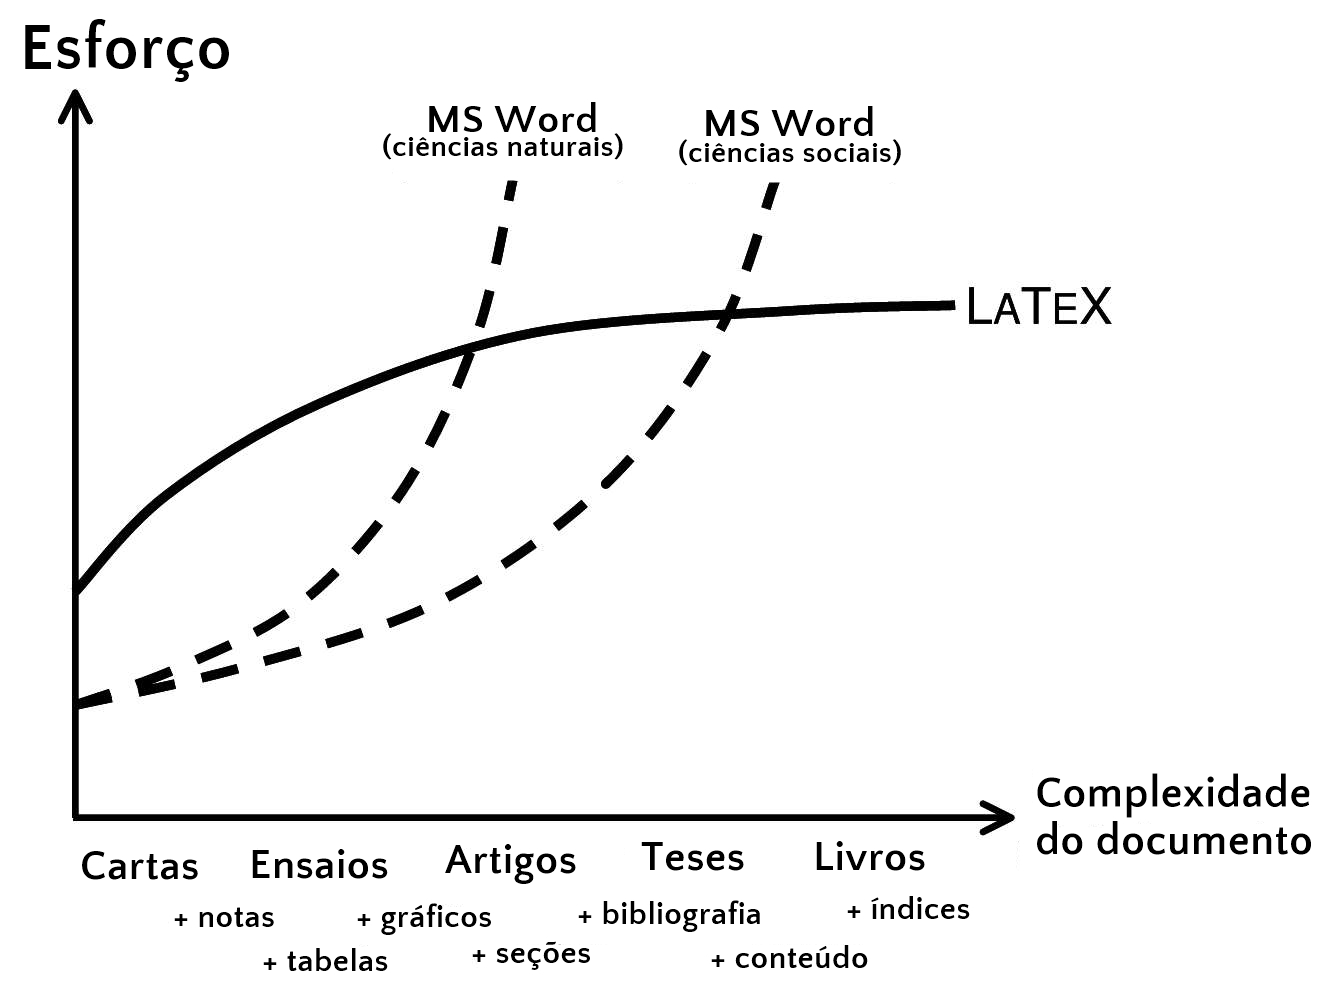
\includegraphics[width=1\textwidth]{AAUgraphics/SFhtj}
%   \input{gdplog.tex}
%    \label{tab:doc-type-cap4} 
%\vspace{0.1cm}
%\small
%\begin{flushleft}
%Fonte: Elaborado pelo autor a partir do processamento de dados da  BM\&FBovespa disponibilizados por \textit{Yahoo Finance} (2018), Tesouro Direto e Banco Central do Brasil.
%\end{flushleft}
\end{figure}
\end{frame}
%#################################################

\begin{frame}{Em resumo:}
\begin{itemize}
\item Alta qualidade tipográfica do documento.
\pause
\item \LaTeX \hspace{0.1cm} permite aos usuários separar claramente o conteúdo do formato do documento.
\pause
\item Isso dá ao usuário a oportunidade de se concentrar em \textquotedblleft qual\textquotedblright \ parte criativa do seu trabalho, e não \textquotedblleft como\textquotedblright \ e nem quando ele será impresso.
\pause
\item É muito simples lidar com equações, figuras, bibliografia e índice.
\pause
\item Programando um pouco de abordagem para colocar as coisas no lugar certo.
\end{itemize}

\end{frame}

%##################################################
\begin{frame}{Motivação}


\begin{center}

\bfseries \Large \LaTeX\hspace{0.01cm}  tem mais flexibilidade em relação ao seu documento e comandos poderosos que facilitam seu trabalho e proporcionam melhores resultados no mínimo tempo.

\end{center}

\end{frame}

%%%%%%%%%%%%%%%%%%%%%%%%%%%%%%%%%%%%%%%%%%%%%%%%%%%%

%%%%%%%%%%%%%%%%%%%%%%%%%%%%%%%%%%%%%%%%%%%%%%%


\section{Tutorial}

\subsection{Setup}

\begin{frame}[fragile]
\frametitle{Configurando o compilador e editor de \LaTeX\vspace{0.2cm}}


\textbf{Para usuários debian, distro. Linux:}\\
Com a conexão à Internet, basta digitar os seguintes comandos um após o outro dentro do terminal de comando:
\begin{itemize}

\item \textsf{sudo apt-get install texlive-full}
\item \textsf{sudo apt-get install texmaker}
\end{itemize}



\textbf{Para usuários Windows:}
\begin{itemize}
\item \href{https://miktex.org/download}{Click Download} e instale MiKTeX.
\item \href{http://www.xm1math.net/texmaker/}{Click Download} e instale Texmaker.
\end{itemize}


\end{frame}

%#############################################

\subsubsection{O Básico}

\begin{frame}[fragile]
\frametitle{Entendendo a estrutura do documento \textsf{*.tex}}


\begin{latexcode}

    % comando usado para ativar o arquivo de design
    \documentclass[Parâmetros globais]{classe.cls}
     
    % comando usado para chamar o pacote necessário
    \usepackage{nome_do_pacote}

    % comando usado para iniciar um documento
    \begin{document}

    % comando usado para finalizar um documento
    \end{document}

    \end{latexcode}
    \end{frame}

%################################################

\begin{frame}{Entendendo os tipos de documentos}
\begin{itemize}
\item article : Para documentos curtos e artigos de revistas.\\ \hspace{1.28cm} Comumente usado!
\item report : Para documentos mais longos e dissertações.
\item book : Útil para escrever livros
\item letter : Útil para escrever cartas
\item beamer : Para apresentações. 
\end{itemize}

\end{frame}

%##################################################

\begin{frame}[fragile]
\frametitle{Conhecendo alguns caracteres reservados}
Os seguintes caracteres de símbolos têm um significado especial: 

\begin{center}
\begin{verbatim}
Caracteres,       Função,         Como digita-lo?

#  Parâmetro de macro,                  \#
$  Modo Matemática,                     \$
%  Commentário,                         \%
^  Sobrescrito(em matemática),          \^{}  
&  Separar as coluna em tabelas,        \&
_  Subscrito(em $ $),                   \_
{} Processar um bloco,                  \{\}
~  Use-o sempre que quiser deixar 
   um espaço inquebrável,               \~{}
\  Iniciar um comando,                  $\backslash$
\end{verbatim}
\end{center}

\end{frame}

%##################################################

\begin{frame}[fragile]
\frametitle{Implementando uma classe para Artigos}

\begin{latexcode}

\documentclass[a4paper, 12pt]{article}

\usepackage[utf8]{inputenc} % codificação
\usepackage[T1]{fontenc}    % símbolos especiais

\usepackage[portuguese]{babel} % idioma

\usepackage{hyphenat} % Regras de hifenização
\hyphenation{mate-mática recu-perar}


\title{Curso introdutório em \LaTeX}
\author{Henrique C. Costa}
\date{2018} % Ignorar data usando \date{}

\begin{document}

\begin{titlepage}
\maketitle
\end{titlepage}
% Agora, comece a preencher seu conteúdo!
\end{document}

\end{latexcode}
\end{frame}

% ##########################################

\begin{frame}[fragile]
\frametitle{Criando ambiente para uso específico}

\begin{latexcode}

...

\begin{document}
...

\begin{} % Preencha o ambiente em {}

% Ambiente criado! 

\end{}

\end{document}

\end{latexcode}
\end{frame}

%###########################################

\begin{frame}{Ambiente}

\begin{minipage}{0.3\linewidth}
\underline{Aligments:}
\begin{itemize}
\item center
\item flushleft
\item flushright

\end{itemize}
\end{minipage}
~
\pause
\begin{minipage}{0.63\linewidth}
\underline{Úteis}
\begin{itemize}
\item tabular{\color{blue}*}
\item table{\color{blue}*}
\item matrix{\color{blue}*}
\item equation{\color{blue}*}
\item minipage{\color{blue} (página pequena na página principal)}
\item verbatim{\color{blue} (para inserir códigos)}
\item itemize{\color{blue}  (ajuda a criar item)}
\item figure{\color{blue}*}

\vspace{0.2cm}
\item[*] {\color{blue} será discutido mais detalhadamente na seção a seguir.}
\end{itemize}
\end{minipage}

\end{frame}

%#############################################


\begin{frame}[fragile]
\frametitle{Comandos úteis}
Aqui estão a lista de comandos: 
\begin{verbatim}
\textbf{bold} \textit{italic} 
{\color{pick} texto_aqui} % Muda a cor do texto 

\vspace{scale} % espaçamento vertical
               % por exemplo: escala = 1cm 
\vspace*{scale} % Para seguir rigorosamente o comando!

\hspace{scale} % para espaçamento horizontal
\hspace*{scale}  
\end{verbatim}
\end{frame}

\begin{frame}[fragile]
\frametitle{Comandos úteis}
 
\begin{verbatim}
\\ significa intervalo (quebra) de linha 
\noindent significa indentação no parágrafo inicial
\underline{texto_aqui} sublinha o texto.

\textquotedblleft  cria aspas duplas esquerda
\textquotedblright cria aspas duplas direita
 
\chapter{•}        cria título de capitulo
\section{•}        cria título de seções
\section*{•}       cria título de seção sem rótulo
\subsection{•}     cria título de sub-seção
\subsubsection{•}  cria título de sub-sub-seção

\end{verbatim}
\end{frame}

\begin{frame}[fragile]
\frametitle{Comandos úteis}
 
\begin{verbatim}

\tableofcontents   cria tabela de conteúdo
\listoffigures     listar todas as figuras rotuladas.
\listoftables      listar todas as tabelas rotuladas.
\newpage           finalizar uma página 
\pagenumbering{*}  pode alterar o estilo de numeração
                   como árabe (1,2, ...) para romano
                   (I, II, ...) colocando
                   ao invés de * 
                    
\end{verbatim}
{\color{blue}Para comandos de matemática, obtê-lo do editor do texmaker!}
\end{frame}

%%%%%%%%%%%%%%%%%%%%%%%%%%%%%%%%%%%%%%%%%%%%%%%%%%%%


%%%%%%%%%%%%%%%%%%%%%%%%%%%%%%%%%%%%%%%%%%%%%%%
\subsection{Construindo algumas habilidades}

\begin{frame}[fragile]
\frametitle{Importação de imagens*}

\begin{latexcode}

...
\usepackage{graphicx}
\graphicspath{{sua_pasta/}{../sua_pasta/}}
% coloque todas as imagens na "sua_pasta" 
% está fora da pasta do seu arquivo LaTeX.
\begin{document}
...

\includegraphics[width = ?cm, height = ?cm]{sua imagem}}

% se você quiser: 
 [scale=?] % imagens em igual proporção em largura e altura
 [angle=?] % Por exemplo: ângulo = 45
\end{document}
\end{latexcode}
{\color{red} *não mostrará na lista de figuras e não pode fazer referência cruzada!}
\end{frame}

%%%%%%%%%%%%%%%%%%%%%%%%%%%%%%%%%%%%%%%%%%%%%%%

\begin{frame}[fragile]
\frametitle{Especificando as posições}
\href{http://ctan.imsc.res.in/macros/latex/contrib/float/float.pdf}{Float*} {\color{blue} é usados para conter contém coisas (ou seja, tabelas e figuras) que devem ser colocadas dentro de uma única página.}
\begin{verbatim}
Parâmetro               Posição
   h           [Coloque o float* aqui, ou seja
               aproximadamente no mesmo lugar
               onde o comando é definido]
   t           [Posição no topo da página]
   b           [Posição na parte inferior da página]
   !           [Substituir os parâmetros internos que
               arquivos de classe usam para determinar 
               a posição de flutuação "boa"]
   H           [Precisamente coloque aqui, no pacote 
               float, é equivalente a h!]
\end{verbatim}

\end{frame}

%##############################################

\begin{frame}[fragile]
\frametitle{Explorar a inserção de imagens}

\begin{latexcode}

...
\begin{document}
\listoffigures
...
\begin{figure}[especificar a posição]

\includegraphics[width = ?cm, height = ?cm]{?imagem}}
\caption{?Será mostrado na lista de figuras!}
\label{fig:?para referência cruzada}

\end{figure}
...\ref{fig:?para referência cruzada}
\end{document}
\end{latexcode}
\end{frame}

%##############################################

\begin{frame}{Algumas sugestões sobre gráficos}
\begin{itemize}
\item Use imagens vetoriais (por exemplo, \textsf{*.ps} e \textsf{*.pdf}) em vez de imagens de quadriculação (por exemplo, \textsf{*.png}) de modo que, a resolução possa estar em boa qualidade.\\
\pause
\vspace{0.2cm}

{\small \bfseries \underline{Imagens vetoriais} são criados em programas de desenho. Este programa usa pontos conectados com curvas ou linhas retas, como conectar-os-pontos. A vantagem de usar essas imagens é que é independente da resolução.\\
Mas, \underline{Raster ou bitmap imagens} usa pixels para definir imagens.}
\pause
\item Não use espaços ao nomear as imagens. 
\pause
\item Escolha nomes de arquivos específicos e descritivos.
\pause
\item Coloque todas as imagens em uma pasta.

\end{itemize}
\end{frame}


%%%%%%%%%%%%%%%%%%%%%%%%%%%%%%%%%%%%%%%%%%%%%%%%%%%%

\begin{frame}[fragile]
\frametitle{Entendendo como funcionam as tabelas}
\begin{verbatim}
Parâmetro          Significado
l            coluna justificada à esquerda
c            coluna centralizada
r            coluna justificada à direita
|            linha vertical
||           linha vertical dupla
&            separador de colunas
\\           iniciar nova linha
\hline       linha horizontal
\end{verbatim}
\end{frame}

%##################################################

\begin{frame}[fragile]
\frametitle{Inserindo tabelas*}
\begin{minipage}{0.5\linewidth}


\begin{latexcode}

...
\begin{document}
...
\begin{tabular}{||c|c||}
\hline
Parâmetro & Significado\\
\hline
l & justificado à esquerda\\
c & coluna centralizada\\
\hline 
\end{tabular}

\end{document}
\end{latexcode}
\end{minipage}
~
\begin{minipage}{0.45\linewidth}
\textbf{Saída:}\\
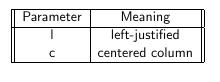
\includegraphics[scale=0.6]{AAUgraphics/table}
\end{minipage}
{\color{red} *não será exibido na lista de tabelas e não pode fazer referência cruzada!}
\end{frame}

%################################################

\begin{frame}[fragile]
\frametitle{Explorando a inserção de tabelas}

\begin{latexcode}
% \begin{document}
\listoftables 
\begin{table}[especificar posição]
\begin{tabular}{||c|c||}
\hline
Parâmetro & Significado\\
\hline
l & justificado à esquerda\\ 
c & coluna centralizada\\ 
% Não esqueceu de adicionar \\ no final
\hline 
\end{tabular}
\caption{?Será mostrado na lista de tabelas!}
\label{table:?para referência cruzada}
\end{table}
... \ref{table:?para referência cruzada}

\end{latexcode}
\end{frame}

%###################################################

\begin{frame}[fragile]
\frametitle{Criando Matrizes}

\begin{minipage}{0.4\linewidth}
\begin{latexcode}
...
\usepackage{amsmath}
%   \begin{document}
...
$\begin{matrix} 
a & b \\
c & d 
\end{matrix}$
...
$
\begin{pmatrix} 
a & b \\
c & d 
\end{pmatrix}$
...

\end{latexcode}
\end{minipage}
~
\begin{minipage}{0.4\linewidth}

\begin{latexcode}
$\begin{bmatrix} 
a & b \\
c & d 
\end{bmatrix}
\quad
\begin{vmatrix} 
a & b \\
c & d 
\end{vmatrix}
\quad
\begin{Vmatrix} 
a & b \\
c & d 
\end{Vmatrix}
$ ...

\end{latexcode}
\end{minipage}

\end{frame}

%##############################################

\begin{frame}{contd.}
\textbf{Saída:}\\
\vspace*{0.2cm}
 
$\begin{matrix} 
\hspace*{0.3cm} a & b \\
\hspace*{0.3cm} c & d 
\end{matrix}
\linebreak 
$
\vspace*{0.2cm}

$\begin{pmatrix} 
a & b \\
c & d 
\end{pmatrix}
\linebreak
$

\vspace*{0.2cm}

$
\begin{bmatrix} 
a & b \\
c & d 
\end{bmatrix}
\quad
\begin{vmatrix} 
a & b \\
c & d 
\end{vmatrix}
\quad
\begin{Vmatrix} 
a & b \\
c & d 
\end{Vmatrix}
$

\end{frame}

%%%%%%%%%%%%%%%%%%%%%%%%%%%%%%%%%%%%%%%%%%%%%%%%%%%%

%%%%%%%%%%%%%%%%%%%%%%%%%%%%%%%%%%%%%%%%%%%%%%%%%%%%

\begin{frame}[fragile]
\frametitle{Inserindo equações}

\begin{latexcode}

\usepackage{amsmath} % pacote importante 

%   \begin{document}
 ... nosso modelo linear:

\begin{equation} \label{eq:eg}
Y_{i} = \alpha + \beta_{1} X_{1i} + \epsilon
\end{equation}

A equação \ref{eq:eg} é conhecida como o método dos 
mínimos quadrados ordinários (MQO).
% Para fazer referências cruzadas, usamos o comando \ ref {}.
Onde $\epsilon$ é termo de erro aleatório 
(variável estocástica) com $\mathbb{E}\epsilon = 0$ 
e ${\bf Var}\epsilon = \sigma^2$.
...

\end{latexcode}
\end{frame}
%############################################
\begin{frame}{contin.}
\textbf{Saída:}
... nosso modelo linear:

\begin{equation} \label{eq:eg}
Y_{i} = \alpha + \beta_{1} X_{1i} + \epsilon
\end{equation}

A equação \ref{eq:eg} é conhecida como o método dos 
mínimos quadrados ordinários (MQO).

Onde $\epsilon$ é termo de erro aleatório 
(variável estocástica) com $\mathbb{E} \epsilon = 0$ 
e ${\bf Var}\epsilon = \sigma^2$.


\end{frame}

%##############################################
\begin{frame}[fragile]
\frametitle{Inserindo equações}

\begin{latexcode}

Nós estimamos $\alpha$ and $\beta_{1}$ 
minimizando a soma dos erros quadrados:

\begin{equation} \label{eq2:eg}
\sum_{i=1}^n (Y_{i} - \alpha - \beta_{1} X_{i})^2
\end{equation}

O {\em valor previsto} ou valor ajustado 

\begin{equation}
\hat Y_{i} = \hat \alpha + \hat \beta_{1} X_{j}
\end{equation}

As diferenças entre as observações $Y_{i}$ 
e os valores ajustado $\hat Y_{i}$ são chamados de 
{\em resíduos} (erros), i.e. 

O estimador MQO do seu vetor \beta \ é:

\begin{equation}
    \hat{\beta} = (X'X)^{-1} X'Y
\end{equation}


\end{latexcode}
\end{frame}
%############################################
\begin{frame}{contin.}
Nós estimamos $\alpha$ and $\beta_{1}$ 
minimizando a soma dos erros quadrados:

\begin{equation} \label{eq2:eg}
\sum_{i=1}^n (Y_{i} - \alpha - \beta_{1} X_{i})^2
\end{equation}

O {\em valor previsto} ou valor ajustado 

\begin{equation}
\hat Y_{i} = \hat \alpha + \hat \beta_{1} X_{j}
\end{equation}

As diferenças entre as observações $Y_{i}$ 
e os valores ajustado $\hat Y_{i}$ são chamados de 
{\em resíduos} (erros), i.e. 

O estimador MQO do seu vetor \beta \ é:

\begin{equation}
    \hat{\beta} = (X'X)^{-1} X'Y
\end{equation}

\end{frame}

%###################################################
%##############################################
\begin{frame}[fragile]
\frametitle{Inserindo equações longas}

\begin{latexcode}

 ...
Por esta definição a função de lucro pode ser expressada
matematicamente da seguinte forma:

\begin{equation}
 \boldsymbol{\pi}\, (p,\textbf{w}) \equiv \; 
 \max_{x \geq 0} \; \; {p \cdot f(x) - \textbf{w} \cdot x} 
\end{equation}

A função lucro transcendental logarítmica (\textit{translog}) 
pode ser descrita matematicamente da seguinte forma:

\begin{equation}
    \begin{split}
 ln \, \boldsymbol{\pi} = \alpha_{0} + \alpha_{1} \, ln \, p +
 \sum_{i} \alpha_{2} \, ln \, \textbf{w}_{i} + \frac{1}{2} \,
 \sum_{i} \, \sum_{j} \beta_{ij} \, ln \, \textbf{w}_{i} \, ln \,
 \textbf{w}_{j} \, \\
 + \sum_{i} \beta_{iy} \, ln \, \textbf{w}_{i} \, ln \, p +
 \frac{1}{2} \, \beta_{yy} \, ln \, p \, ln \, p  
\end{split}
\end{equation}

\end{latexcode}
\end{frame}
%############################################
\begin{frame}{Inserindo equações longas}
 ...
Por esta definição a função de lucro pode ser expressada matematicamente da seguinte forma:

\begin{equation}
 \boldsymbol{\pi}\, (p,\textbf{w}) \equiv \; \max_{x \geq 0} \; \; {p \cdot f(x) - \textbf{w} \cdot x} 
\end{equation}

A função lucro \textit{translog} pode ser descrita matematicamente da seguinte forma:

\begin{equation}
    \begin{split}
 ln \, \boldsymbol{\pi} = \alpha_{0} + \alpha_{1} \, ln \, p + \sum_{i} \alpha_{2} \, ln \, \textbf{w}_{i} + \frac{1}{2} \, \sum_{i} \, \sum_{j} \beta_{ij} \, ln \, \textbf{w}_{i} \, ln \, \textbf{w}_{j} \, \\
+ \sum_{i} \beta_{iy} \, ln \, \textbf{w}_{i} \, ln \, p + \frac{1}{2} \, \beta_{yy} \, ln \, p \, ln \, p  
\end{split}
\end{equation}

\end{frame}

%###################################################
%%%%%%%%%%%%%%%%%%%%%%%%%%%%%%%%%%%%%%%%%%%%%%%%%%%%

\begin{frame}[fragile]
\frametitle{Bibliografia: Bibtex}
Criaremos bibliografia usando o Bibtex em vez do ambiente de bibliografia({\color{brown}\href{https://www.sharelatex.com/learn/Bibliography_management_with_bibtex}{se você quiser, click agora!}}). Aqui estão os seguintes passos:

\begin{itemize}
\item Crie um novo arquivo no Share\LaTeX.
\item Dentro de um projeto, click em {\color{blue}novo arquivo} dê um rótulo, e coloque a extensão {\color{blue}Bibtex} {\color{red}.bib}.
\item Escolha o tipo de documento que deseja citar. Por exemplo: \textquotedblleft Artigo em uma Revista\textquotedblright.
\item Então, você verá como:

\end{itemize}

\end{frame}

%%%%%%%%%%%%%%%%%%%%%%%%%%%%%%%%%%%%%%%%%%%%%%%


\begin{frame}[fragile]
\frametitle{cont.}
\begin{latexcode}
@Article{*, % Esta linha * significa rótulo para citações.
author = {*},
title = {*},
journal = {*},
year = {*},
key = {*},    % opcional
volume = {*}, % se você quiser colocar o volume então,
number = {*}, % Se você não precisar disso, basta removê-lo.
pages = {*},
month = {*},  % nunca esqueça "vírgula"
note = {*},
annote = {*}  
}
\end{latexcode}
\end{frame}

%#############################################

\begin{frame}[fragile]
\frametitle{cont.}

\begin{itemize}
\item Preencha as informações como:
\end{itemize}
\begin{latexcode}
@article{christensen1973,
  title={Transcendental logarithmic production frontiers},
  author={Christensen, Laurits R and Jorgenson, Dale W and Lau, Lawrence J},
  journal={The review of economics and statistics},
  pages={28--45},
  year={1973},
  publisher={JSTOR}
}

@book{gujarati2009,
  title={Basic Econometrics},
  author={Gujarati, Damodar N},
  year={2009},
  publisher={Tata McGraw-Hill Education}
}
\end{latexcode}
{\color{red}Remova os itens que não são usados!}
\end{frame}


%###############################################
\begin{frame}{Buscando bib no Google Acadêmico}
\begin{figure}
%    \centering
    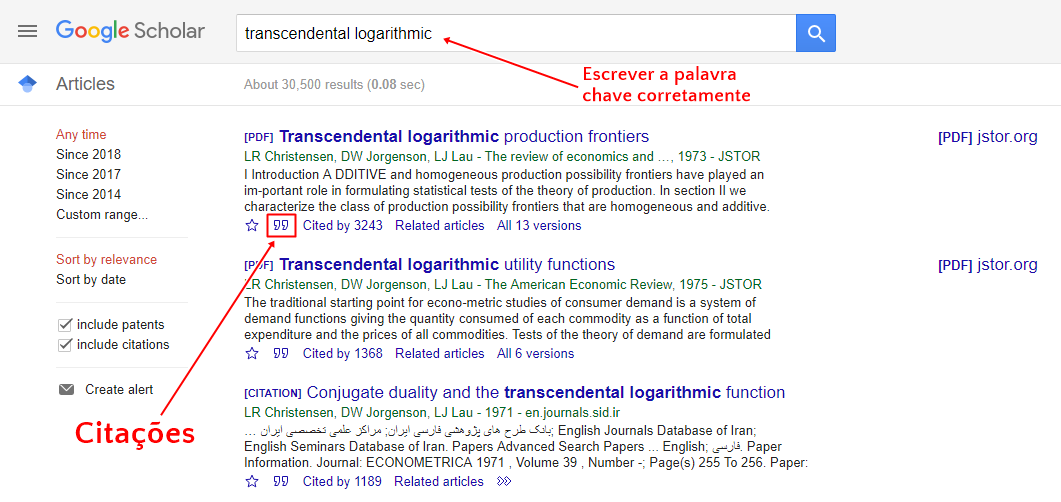
\includegraphics[scale=0.35]{AAUgraphics/bib01}
%    \caption{Caption}
%    \label{fig:my_label}
\end{figure}
\end{frame}

%###############################################
%###############################################
\begin{frame}{Buscando bib no Google Acadêmico}
\begin{figure}
%    \centering
    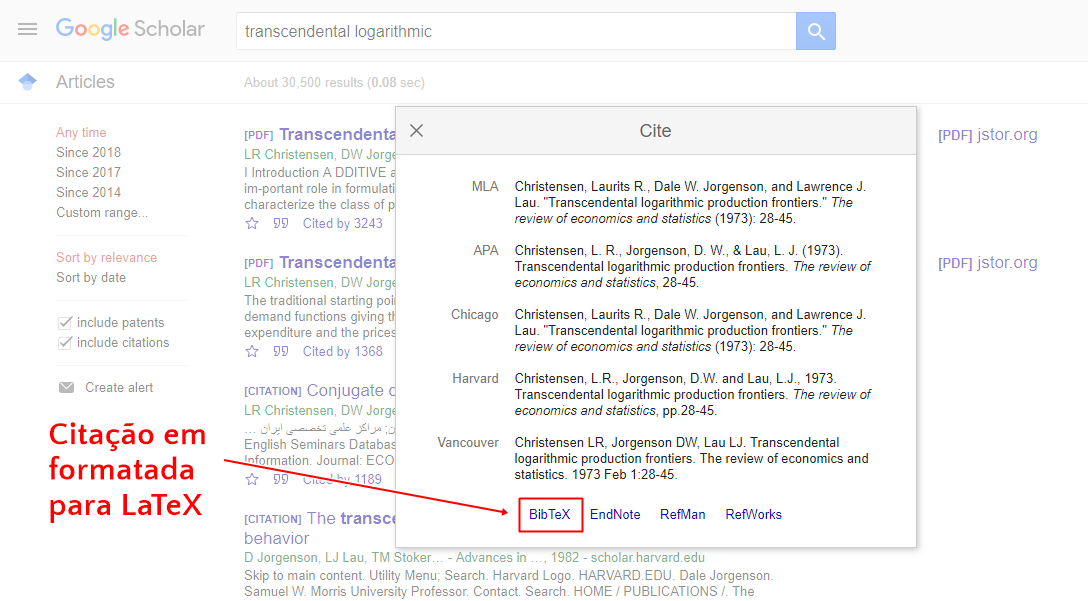
\includegraphics[scale=0.34]{AAUgraphics/bib02}
%    \caption{Caption}
%    \label{fig:my_label}
\end{figure}
\end{frame}

%###############################################
%###############################################
\begin{frame}{Buscando bib no Google Acadêmico}
\begin{figure}
%    \centering
    
\includegraphics[scale=0.58]{AAUgraphics/bib03}
%    \caption{Caption}
%    \label{fig:my_label}
\end{figure}
\end{frame}

%###############################################
%%%%%%%%%%%%%%%%%%%%%%%%%%%%%%%%%%%%%%%%%%%%%%%

\begin{frame}{Lista de pacotes úteis*}
\begin{itemize}
\item comment {\color{blue}(ajuda a criar um comentário multilinha)*}
\item float    {\color{blue}(coloca os gráficos na posição desejada)*}
\item imakeidx {\color{blue}(Cria índices)*}
\item nomencl  {\color{blue}(Cria lista de abreviações)*}
\item geometry {\color{blue}(ajuda a modificar o layout)}
\item hyperref {\color{blue}(usar para criar hiperlink)}
\item fancyhdr {\color{blue}(Use para design de cabeçalho e rodapé)}
\item mathptmx {\color{blue}(para  \href{http://ctan.org/pkg/mathptmx}{\color{brown}Times New Roman})}

\vspace{0.2cm}
\item[*] {\color{blue} será discutido mais detalhadamente na seção a seguir.}

\end{itemize}
\end{frame}
%################################################

%################################################
\section{Mais sobre \LaTeX}
\begin{frame}{Referencias }
Aqui estão a lista de recursos onde eu aprendi muitas coisas em \LaTeX.
\begin{itemize}
\item \href{https://www.sharelatex.com/learn/}{ShareLaTeX}
\item \href{https://tex.stackexchange.com/}{\TeX\hspace{0.1cm} Stack Exchange}
\item \href{https://www.overleaf.com/latex/templates}{Overleaf}
\item \href{https://www.overleaf.com/latex/templates}{Wikibooks}

\end{itemize}
\end{frame}
%###############################################

%###############################################
\begin{frame}{Palavras finais !!!}

\begin{center}
\textbf{{\large \underline{Tarefa}}\\
Mantenha este arquivo de apresentação\footnote{Este arquivo de apresentação é preparado usando beamer \LaTeX\hspace{0.1cm}. Encontre uma cópia do código fonte em \url{https://github.com/Henrikun/LaTeX}} como um guia!\\
Crie um documento \LaTeX\hspace{0.1cm} vazio e implemente todos os materiais que você aprendeu hoje!}\\
\vspace{1cm}

\end{center}
\end{frame}


%HURRAY! I FINALLY DID IT!


%%%%%%%%%%%%%%%%
%\section{Feedback}
%\subsection{Contato e Informações}
% contact information
%\begin{frame}{Feedback}{Contato e Informações}
%Em caso de comentários, dúvidas e sugestões, por favor não hesitar em me contactar.

%  \begin{center}
 %   \insertauthor\\
  %  \chref{http://lattes.cnpq.br/6259049914329971}{http://lattes.cnpq.br/6259049914329971}\\
     
     
 % \end{center}
%\end{frame}
%%%%%%%%%%%%%%%%

{\aauwavesbg%
\begin{frame}[plain,noframenumbering]%
  \finalpage{\Large OBRIGADO PELA SUA ATENÇÃO}
\end{frame}}
%%%%%%%%%%%%%%%%

\end{document}
